%15-21 de la lista 1 y el 12 de la lista 2
\begin{enumerate}
	\setcounter{enumi}{14} 
	\item Se tira un par de dados. Si la suma de los dos es cuando menos igual a 7. Calcule la probabilidad de que sea igual a 9.
    \\\textbf{Solución}
    
    \begin{gather*}
    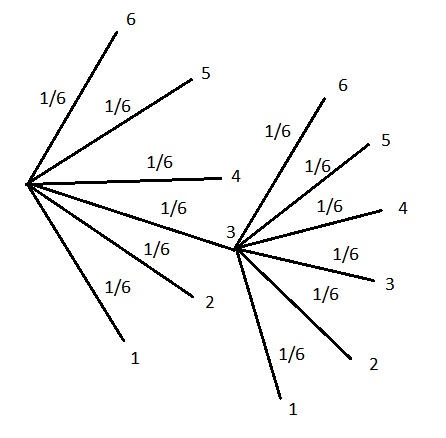
\includegraphics{imagenes/problema15}\\
       P(7\geq) = \frac{1}{6}[\frac{1}{6}(1+2+3+4+5+6)]=\frac{21}{36}\\
        P(9) = \frac{4}{36}\\
        P(9|7\geq) = \frac{P(9|7\geq)}{P(7\geq)} = \frac{\frac{4}{36}}{\frac{21}{36}} = \frac{4}{21}\text{ ó } 19.04\%
    \end{gather*}
	\item Supongamos que 5 de cada 100 hombres y 25 de cada 10000 sufren daltonismo.\\
	Una persona daltónica se escoge aleatoriamente.\\
	¿Cuál es la probabilidad de que sea hombre? (Supongamos que hay el mismo número de hombres que de mujeres)
    \\\textbf{Solución}
      \begin{gather*}
        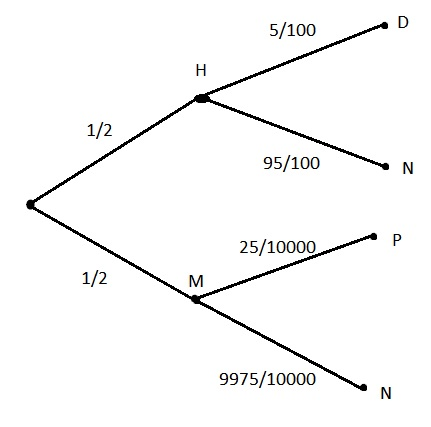
\includegraphics{imagenes/problema16}\\
           P(D) = (\frac{1}{2})(\frac{5}{100})+(\frac{1}{2})(\frac{25}{10000})=\frac{525}{20000}\\
            P(H|D) = \frac{P(H \cap D)}{P(D)} = \frac{\frac{500}{20000}}{\frac{525}{20000}} = \frac{500}{525} = \frac{20}{21} \text{ ó } 95.23\%
    \end{gather*}
	\item Se escoge al azar un punto entre el 0 y el 1 en el eje de las x dentro del plano(x,y).\\A continuación se dibuja un circulo con centro en el origen y radio determinado por el punto escogido.\\Calcula la probabilidad de que el área del circulo sea menor que $\pi$/2
    \\\textbf{Solución}
    \begin{gather*}
        \pi r^{2}=\frac{\pi}{2}\\
        r=\frac{1}{\sqrt{2}}\\
        p(A) = \frac{\frac{1}{\sqrt{2}}}{1}=\frac{1}{\sqrt{2}} \text{ ó } 70.71\%
    \end{gather*}
	\item Se rompe una regla de 12 pulgadas al azar en 2 partes a lo largo.\\
	¿Cuál es la probabilidad de que la longitud de la parte más larga sea al menos el doble de la corta?
    \\\textbf{Solución}
    \begin{gather*}
        x + y = 12\\
        y = \frac{x}{2}\\
        x + \frac{x}{2} = 12\\
        x = 8\\
        L = 12 - 8 = 4*2 = 8\\
        P(L)=\frac{8}{12}=\frac{2}{3}
    \end{gather*}
	\item Si la función de probabilidad de la variable aleatoria y esta dada por:
	\begin{gather*}
	    f(y)= \left\{ \begin{array}{lcc}
             \frac{1}{8}(y+1) & 2 \leq y \leq 4\\
             \\ 0 & otro 
             \end{array}
   \right.
	\end{gather*}
    \\\textbf{Solución}
    \\\text{La variable es continua}
    \begin{gather*}
        P(\Omega)=1\\ 
    \end{gather*}
       \[ \int_{2}^{4}  \! F(y) \, dy =
        \int_{2}^{4}  \! \frac{1}{8}(y+1) \, dy =\frac{1}{8}\int_{2}^{4}  \! (y+1) \, dy = 
        \]
    \begin{gather*}
    \frac{1}{8}(\frac{y^2}{2}+y)|_2^4 =
        \frac{1}{8}[(8+4)-(2+2)]\frac{1}{8}(8)=1 \\
    \end{gather*}
\\\textbf{Determine}\\
     \begin{enumerate}
           \item P(y $<$ 3.2)\\
            \item P(2.9 $<$ y $<$ 3.1)
        \end{enumerate}
      \begin{enumerate}
           \item  \[\frac{1}{8}\int_{2}^{3.2}  \! (y+1) \, dy =\frac{1}{8}(\frac{y^2}{2}+y)|_2^3.2 = \frac{1}{8}[(5.12+3.2)-(2+2)]=\frac{1}{8}[8.32-4]
    \]
    \[=\frac{4.32}{8}=54\% 
        \]
        \item \[\frac{1}{8}\int_{2.9}^{3.2}  \! (y+1) \, dy =\frac{1}{8}(\frac{y^2}{2}+y)|_2.9^3.2 = \frac{1}{8}[(5.12+3.2)-(4.205+2.9)]
    \]
    \[=\frac{1}{8}[1.215]=15.1875\% 
        \]
        \end{enumerate}
	\item Si la función de distribución de la variable aleatoria x está dada por
	\begin{gather*}
	    f(y)= \left\{ \begin{array}{lcc}
             \frac{c}{\sqrt{x}} & 0 \leq x \leq 4\\
             \\ 0 & otro 
             \end{array}
   \right.
	\end{gather*}
	Determine el valor de c\\
    \\\textbf{Solución}
    \\\text{La variable es continua}
    \begin{gather*}
        P(\Omega)=1\\ 
    \end{gather*}
       \[ \int_{0}^{4}  \! \frac{c}{\sqrt{x}} \, dx =
        c\int_{0}^{4}  \! \frac{1}{\sqrt{x}} \, dx 
        \]
    "No se puede integrar"
    \[ \frac{1}{\sqrt{0}}
    \] No existe
	\item La cantidad real de café (en gramos) en un recipiente de 230 gr llenado por cierta máquina es una variable aleatoria cuya densidad de probabilidad está dada por
	\begin{gather*}
	    f(y)= \left\{ \begin{array}{lcc}
             0 & x \leq 227.5\\
             \\ \frac{1}{5} & 227.5 < x < 232.5 \\
             \\ 0 & x \geq 232.5
             \end{array}
   \right.
	\end{gather*}
	Determine la probabilidad de que en un recipiente de 230gr llenado por esta máquina contendrá cuando mucho 228.65gr de café
    \\\textbf{Solución}
     \\\text{La variable es continua}
    \begin{gather*}
        P(\Omega)=1\\ 
    \end{gather*}
       \[ \int_{227.5}^{232.5}  \! \frac{1}{5} \, dx =
        \frac{1}{5}\int_{227.5}^{232.5}  \! \frac{1}{5} \, dx = \frac{1}{5}x |_{227.5}^{232.5}
        \] 
    \begin{gather*}
    \frac{5}{5}=1
    \end{gather*}
   \[ \int_{227.5}^{228.65}  \! \frac{1}{5} \, dx = \frac{1}{5}x |_{227.5}^{228.65} = \frac{1}{5}(228.65-227.5)
        \] 
    \[=\frac{1}{5}(1.15)= 0.23 \text{ ó} 23\% 
        \]
\end{enumerate}
12. Suponga que el 40\% de los empleados a destajo de la empresa ACME están a favor de tener representación sindical y que se entrevista a una muestra aleatoria de 10 de ellos y se les solicita una respuesta anónima.\\¿Cuál es la probabilidad de que la mayoria de los que respondan estarán a favor de la representación sindical?
\\\textbf{Solución}
\\\text{La variable es de poisson}
\begin{gather*}
    \lambda=np=(10)(0.4) = 4\\
    x>6\\
    P(x) =1-\sum _{x=0}^{5}\frac{{\lambda}^{x}{e}^{-\lambda}}{x!}=1 - \sum _{x=0}^{5}\frac{{4}^{x}{e}^{-4}}{x!} =  0.214869613 \text{ ó } 21.48\%
\end{gather*}